\documentclass[a4paper, 11pt]{report}
\usepackage{graphicx}
\usepackage{xcolor} % colors
\usepackage{lipsum}
\usepackage{fancyhdr} % used for header customization
\usepackage{todonotes}
\usepackage{ifthen} % used to toggle commands on or off
\usepackage{parskip}
\usepackage{cite}

\usepackage{listings} % for code snippets

% code style for error messages
\lstdefinestyle{compilation_error}{
    language=text, % Specify plain text
    backgroundcolor=\color{lightgray}, % Gray background
    numbers=none, % No line numbers
    frame=none,   % No frame
    basicstyle=\ttfamily\footnotesize, % Typewriter font, small size
    breaklines=true, % Allow text to wrap
    showstringspaces=false, % Don't show spaces in strings
    captionpos=b, % Caption at bottom (though we won't use one)
    % Removed options like caption and label to ensure none appear
}

\definecolor{mGreen}{rgb}{0,0.6,0}
\definecolor{mGray}{rgb}{0.5,0.5,0.5}
\definecolor{mPurple}{rgb}{0.58,0,0.82}
\definecolor{backgroundColour}{rgb}{0.95,0.95,0.92}
\definecolor{codeblue}{rgb}{0.2,0.2,0.8} % A nice blue for function names

\lstdefinestyle{CStyle}{
    backgroundcolor=\color{backgroundColour},
    % commentstyle=\color{mGreen},
    % keywordstyle=\color{magenta},
    % numberstyle=\tiny\color{mGray},
    % stringstyle=\color{mPurple},
    basicstyle=\ttfamily\footnotesize,
    breakatwhitespace=false,         
    breaklines=true,                 
    captionpos=b,                    
    keepspaces=true,                 
    numbers=left,                    
    numbersep=5pt,                  
    showspaces=false,                
    showstringspaces=false,
    showtabs=false,                  
    tabsize=2,
    language=C,
    % frame=single,
    rulecolor=\color{mGray}, % frame color
    aboveskip=1.5ex, % Space above listing
    belowskip=1.5ex, % Space below listing
    framesep=4pt, % Space between code and frame
        % --- New additions for blue function names ---
    emph={init, free, get, find, insert, to_evict, evict, remove}, % List your C function names here
    emphstyle=\color{codeblue}\bfseries, % Apply bold blue to the listed names
}


% makes citations clickable
\usepackage{hyperref}
\hypersetup{
    colorlinks=true, % Makes the links colored instead of boxed
    linkcolor=blue,  % Color for internal links (e.g., table of contents, citations)
    citecolor=darkred,  % Color for citation links
    urlcolor=blue,   % Color for URL links
    filecolor=magenta, % Color for file links
    bookmarks=true,  % Adds PDF bookmarks for sections, etc.
    bookmarksnumbered=true, % Numbers the bookmarks
    pdfpagemode=UseOutlines % Opens PDF with bookmarks panel open
}

\usepackage{cleveref} % adds "Figure" or whatever infront

% custom colors
\definecolor{darkred}{rgb}{0.7,0,0}
\definecolor{lightgray}{rgb}{0.96,0.96,0.96}

% numbered subsections
\setcounter{secnumdepth}{3}

\newcommand{\todolaura}[1]{\todo[inline, color=purple!30]{#1}}

\newcommand{\reminder}[1]{\todo[inline, color=orange!30]{#1}} % import custom commands

% correctly format quotations
\usepackage[autostyle, english = american]{csquotes}
\MakeOuterQuote{"}


\renewcommand{\chaptername}{} % remove "chapter" from chapter headings

\textwidth 15cm
\textheight 22cm
\oddsidemargin 0.85cm
\evensidemargin 0.37cm

% Show outline --------------
\newboolean{showoutline}
\setboolean{showoutline}{true}  % Change to false to hide
% ---------------------------

\begin{document}
\thispagestyle{empty}

\begin{center}
\vspace{1mm}

\includegraphics[height=28mm]{resources/logo-vua.pdf}
\vspace{1cm}

{\Large Bachelor Thesis}
\vspace{1cm}

\rule{.9\linewidth}{.6pt}\\
\vspace{0.4cm}
{\huge \bfseries A Comparative Study of Cache Primitives Across Diverse \\ Workload Distributions \par}
\vspace{0.4cm}
\rule{.9\linewidth}{.6pt}\\[1.5cm]
\vspace*{2mm}
{\Large

\begin{tabular}{l}
{\bf Author:} Laura Stampf (2701672)
\end{tabular}
}

\vspace*{1.5cm}

\begin{tabular}{ll}
{\it 1st supervisor:} & Wan Fokkink \\
{\it 2nd reader:} & Femke van Raamsdonk  \\
\end{tabular}

\vspace*{2cm}
\textit{A thesis submitted in fulfillment of the requirements for\\ the VU Bachelor
of Science degree in Computer Science }
\vspace*{1cm}

\today % Date
\end{center}

\pagestyle{fancy}
%... then configure it.
\fancyhead{} % clear all header fields
% \fancyhead[R]{meow \chaptername}
\fancyhead[R]{ \leftmark}

\newpage\begin{abstract}
    \lipsum[1-4]
\end{abstract}
\tableofcontents

% Testing citations ----------------------
\TODO{\textbf{Testing citations}

Sieve citation\cite{sieve}

Web caching overview citation\cite{web-cache-overview}

S3-FIFO citation\cite{s3-fifo}}


% ----------------------------------------

\newpage\chapter{Introduction}

\outline{What is the cache and why is it important}

Sieve citation\cite{sieve}

Web caching overview citation\cite{web-cache-overview}

S3-FIFO citation\cite{s3-fifo}

\lipsum[1]

\outline{How does the cache decide what to evict => introduce cache eviction policies}

\lipsum[1]

\outline{Different types of cache eviction algorithms. Not all are used in practice}

\lipsum[1]

\outline{}
\newpage\chapter{Background and Related Work}

\lipsum

Some text \cite{test}
\newpage\chapter{Design and Implementation}

To answer the main research question of this work (posed in \Cref{sec: research_q}), several crucial design choices had to be made. The following three questions tackle each of these decisions:

\begin{enumerate}
    \item \textbf{Cache simulations}: how to benchmark cache eviction algorithms against different workloads.
    \item \textbf{Eviction algorithms}: the kind of cache eviction algorithms to benchmark.
    \item \textbf{Workloads}: the kind of workloads to use.
\end{enumerate}


The implementation of and motivation for each of these design choices is tackled in the following sub-sections, \Cref{sec: cache-simulations,sec: cache-eviction-algs,sec: workloads}.

\section{Cache simulator}\label{sec: cache-simulations}

\outline{What simulation library used and why?}

The building and execution of cache simulations was performed using the cache simulator provided by \textbf{libCacheSim}\footnote{GitHub for libCacheSim library: \url{https://github.com/1a1a11a/libCacheSim}}, a high-performance open-source library specifically designed for cache simulation and trace analysis. This tool was chosen due to its simple extensibility of new algorithms and support for various workload formats, including CSV, BIN, TXT, and VSCSI files. 

\subsection{Alternative cache simulators}

For the execution of cache simulations, it was crucial to find an open-source cache simulator that supported specifying the cache eviction algorithm with which to evaluate performance on a given web workload. The libCacheSim library's strength lies in its detailed documentation on how to extend the framework with eviction algorithms or trace readers \footnote{Markdown file describing extendability of libCacheSim: \url{https://github.com/1a1a11a/libCacheSim/blob/develop/doc/advanced_lib_extend.md}}.


many other cache simulators exist but many for hardware caches. important to specify that this work focuses on software caches, specifically web caches. aws highlights different kinds of software caches that are used in the context of web services (dns,

\url{https://aws.amazon.com/caching/#topic-0}

CacheSim\footnote{\url{https://github.com/yxchencs/CacheSim}} with research paper \cite{cachesim}

Cache Simulator:
"A state-of-the-art cache and memory hierarchy simulator featuring advanced prefetching, multi-processor support, and comprehensive performance analysis tools."
\url{https://github.com/muditbhargava66/CacheSimulator}


\TODO{why was this tool chosen?}

\TODO{what alternatives exist?}



\subsection{Setup issues with libCacheSim}

It is notable that the open-source libCacheSim library, written in C/C++, has been developed primarily for Ubuntu 22.04 systems reliant on GCC (GNU Compiler Collection) for compilation. Due to this, there were many compatibility issues when setting up the library on the device used for development: an Apple MacBook Pro M1 reliant on the Clang compiler. As part of the effort of this work and as a contribution to the open-source project, many of these issues have been addressed, and GitHub pull requests \footnote{The following pull requests were made to the libCacheSim project: \url{https://github.com/1a1a11a/libCacheSim/pull/179}, \url{https://github.com/1a1a11a/libCacheSim/pull/181}, \url{https://github.com/1a1a11a/libCacheSim/pull/183}} have been made to improve the open-source project's cross-compatibility.

Most issues were caused by an unsuccessful compilation on the macOS device. A major cause of this incompatibility stems from differences in compiler strictness (GCC vs. Clang) - Clang is known for being very strict and pedantic with its warnings, especially concerning potential portability issues or undefined behavior\cite{llvm_diagnostics}, causing many warnings silenced by GCC to be flagged as errors on Clang.

Some interesting issues and discoveries related to cross-compatibility found in the libCacheSim codebase are briefly addressed below.

\begin{description}
    \item[Format specifier mismatches] 
    
    The libCacheSim codebase contains many \code{printf} statements for logging various details, such as the miss ratio of a single cache simulation run. A specific issue encountered was related to the non-portable use of format specifiers. Specifically, for variables of type \code{int64\_t} (signed 64-bit integer), the \code{\%ld} format specifier was used. This is a reasonable usage for Ubuntu (with GCC), but is an incorrect format specifier for macOS (with Clang), which expects \code{int64\_t} variables to use \code{\%lld} instead. This specific format string mismatch caused a compilation error on macOS, specifying the following issue:

    \lstset{style=compilation_error}
    
    \begin{lstlisting}
format specifies type `long' but the argument has type `int64_t' (aka `long long')
    \end{lstlisting}

    A naive solution to this compatibility issue could be wrapping \code{printf} statements with \enquote{problematic} format specifiers in preprocessor macros (i.e. \code{\#ifdef}, \code{\#if defined}, or \code{\#if}) to detect the operating system or compiler. However, this method adds conditional compilation complexity and makes maintenance so much more difficult. Instead, the optimal solution to ensure cross-compatibility lies within the \code{<inttypes.h>} header, where special format macros are defined that expand to the correct format specifier depending on the compilation platform. In the case of the \code{int64\_t} type, which requires format specifier \code{\%ld} on Ubuntu but \code{\%lld} on macOS, the \code{PRId64} macro can be used as a portable solution to the format specifier mismatch. The PRId64 macro is part of a family of macros known as format string macros for fixed-width integers introduced in the C99 standard \cite{cppreference_inttypes} to address these kinds of portability issues.
    

    \item[Unsupported linker options]


    
    \item[Path-dependent package manager]
\end{description}



% LibCacheSim also provides a rich set of features, including state-of-the-art eviction and admission algorithms, out-of-the-box parallelism, and comprehensive trace analysis functionalities, making it a robust and versatile solution for in-depth cache performance studies. Its simple API and extensibility further streamline the process of building complex cache hierarchies and integrating new algorithms.




\outline{Describe setup process}





\section{Cache eviction algorithms}\label{sec: cache-eviction-algs}

To support the proper execution of a cache eviction algorithm, the libCacheSim simulator used in this work requires the implementation of eight methods for a newly added cache eviction algorithm, given by \cref{code: cache-functions}.

\lstset{style=CStyle}

\begin{lstlisting}[language=C, caption=Functions required for cache eviction algorithms in libCacheSim, label=code: cache-functions]
cache_t *init(const common_cache_params_t ccache_params, const char *cache_specific_params);

void free(cache_t *cache);

bool get(cache_t *cache, const request_t *req);

cache_obj_t *find(cache_t *cache, const request_t *req, const bool update_cache);

cache_obj_t *insert(cache_t *cache, const request_t *req);

cache_obj_t *to_evict(cache_t *cache, const request_t *req);

void evict(cache_t *cache, const request_t *req);

bool remove(cache_t *cache, const obj_id_t obj_id);
\end{lstlisting}

Seeing as all of these methods use parameters with types specific to the library itself (i.e. \code{{common\_cache\_params\_t}}), it was crucial first to study the behavior and usage of these in the framework.

\subsection{SIEVE}

\subsection{LRU}

\subsection{FIFO}

\section{Workloads}\label{sec: workloads}}

synthetic data

zipf

used relative measurements to make it scalable in some sense

\section{Experimental setup}

how big is a cache usually?

looked at sieve paper to calculate percentages of unique requests in the traces they used

\TODO{USING AUTO: "cachesim can detect the working set of the trace and automatically generate cache sizes at 0.0001, 0.0003, 0.001, 0.003, 0.01, 0.03, 0.1, 0.3 of the working set size. You can enable this feature by setting cache size to 0 or auto."}
\newpage\chapter{Results}\label{chapter:results}

This chapter discusses the experimental results. First, some notable insights and results from the synthetic Zipf-like workload generation are explored in \Cref{res:zipf-gen}. Then, we dive into the most relevant findings of this work, regarding the cache simulations performed in \Cref{res:cache-sim}.

\section{Synthetic Data Generation}\label{res:zipf-gen}

This section examines some insights gained from generating the synthetic Zipf-like workloads used to simulate web traffic for the cache simulations.

\subsection{Theoretical Zipfian Distributions}\label{theoretical-zipf}

As previously discussed in \Cref{bkg: zipfian-distributions}, Zipfian distributions are characterized by the skewness parameter $\alpha$, which dictates the frequency with which a few popular items are accessed compared to a vast number of less popular items. Lower values of $\alpha$ result in a more uniform distribution where all items have nearly equal probability of being accessed. When $\alpha=1$, the probability of accessing an item is exactly inversely proportional to its rank. For $\alpha>1$, the distribution becomes more heavily skewed; the most popular items are accessed dramatically more often, and the long tail of unpopular items becomes even flatter and less likely to be requested. 

The effect of the skewness parameter $\alpha$ is best visualized by the rank-frequency plots in \Cref{fig:zipf-alpha}. The linear plot demonstrates the shape of Zipfian distributions; items with a lower rank have a higher probability of being sampled. We observe from the log plot that the relationship between rank and probability is a straight line, confirming the inverse power-law relation inherent in a Zipfian distribution. The slope of each line is directly related to the $\alpha$ value; a larger negative slope corresponds to a larger $\alpha$, and a shallower negative slope corresponds to smaller values. This visually demonstrates how $\alpha$ controls the decay rate of the distribution, with a higher value indicating that the probability drops off more quickly with increasing rank.


\begin{figure}[h!]
    \centering
    \caption{Rank-Frequency Plots for Zipfian Distributions (linear and log scales)}
    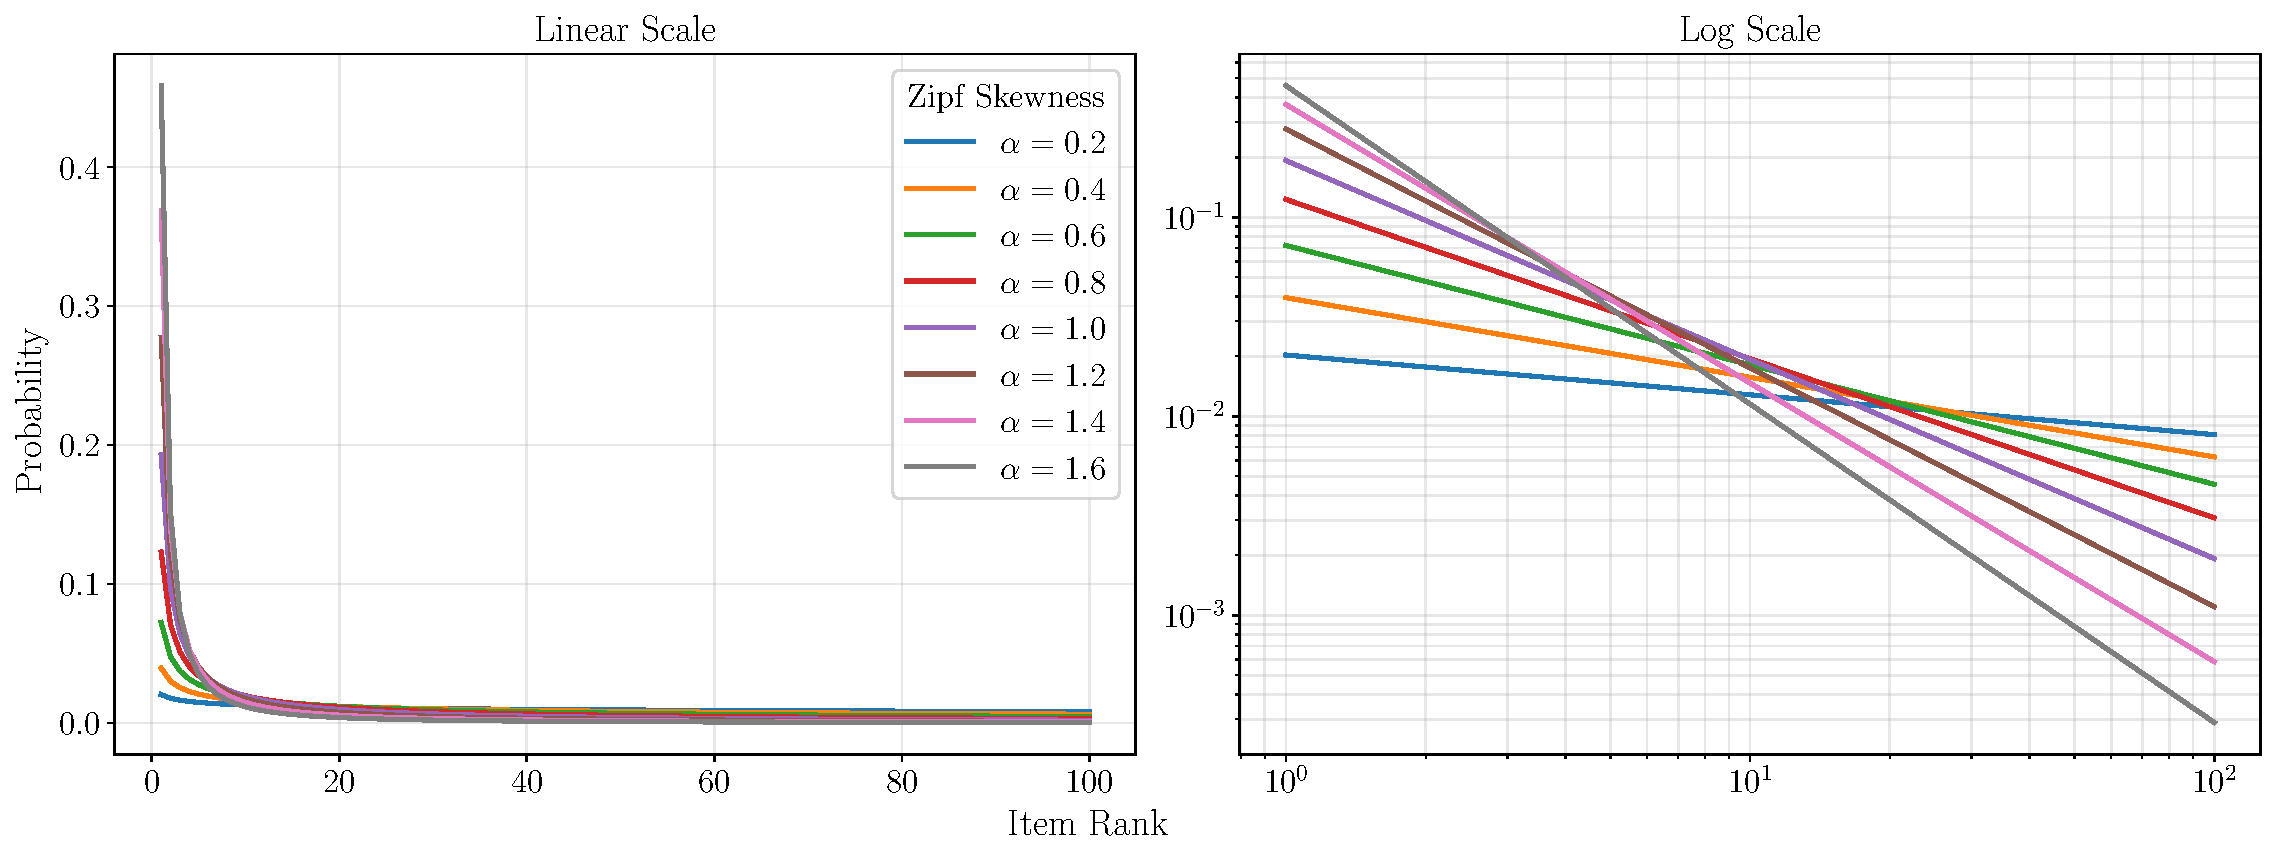
\includegraphics[width=\linewidth]{figures/workloads/zipfian_curves_all_both_no_title.pdf}
    \label{fig:zipf-alpha}
\end{figure}

\subsection{Actual Zipf-like Workloads Generated}

The generated Zipf-like workloads were sampled from Zipfian distributions with differences in (1) skewness parameter $\alpha$ and (2) working set size, which is the set of unique requested items (see \Cref{subsec: synthetic-data-generation}). Due to the probabilistic nature of sampling, the size of the actual working set of the generated workloads differs from the target working set indicated at sampling time. In fact, the difference between the two shows to have been heavily impacted by the choice in $\alpha$, as can be seen from the boxplot in \Cref{fig:boxplot-actual-theoretical-ratio}.

\begin{figure}[h!]
    \centering
    \captionsetup{justification=centering}
    \caption{Boxplot of Actual/Theoretical Working Set Ratio By Zipfian Skewness Parameter $\alpha$. The {\color{PineGreen}\textbf{green}} line represents the median and the {\color{blue}\textbf{blue}} box represents the interquartile range (middle 50\% of data).}
    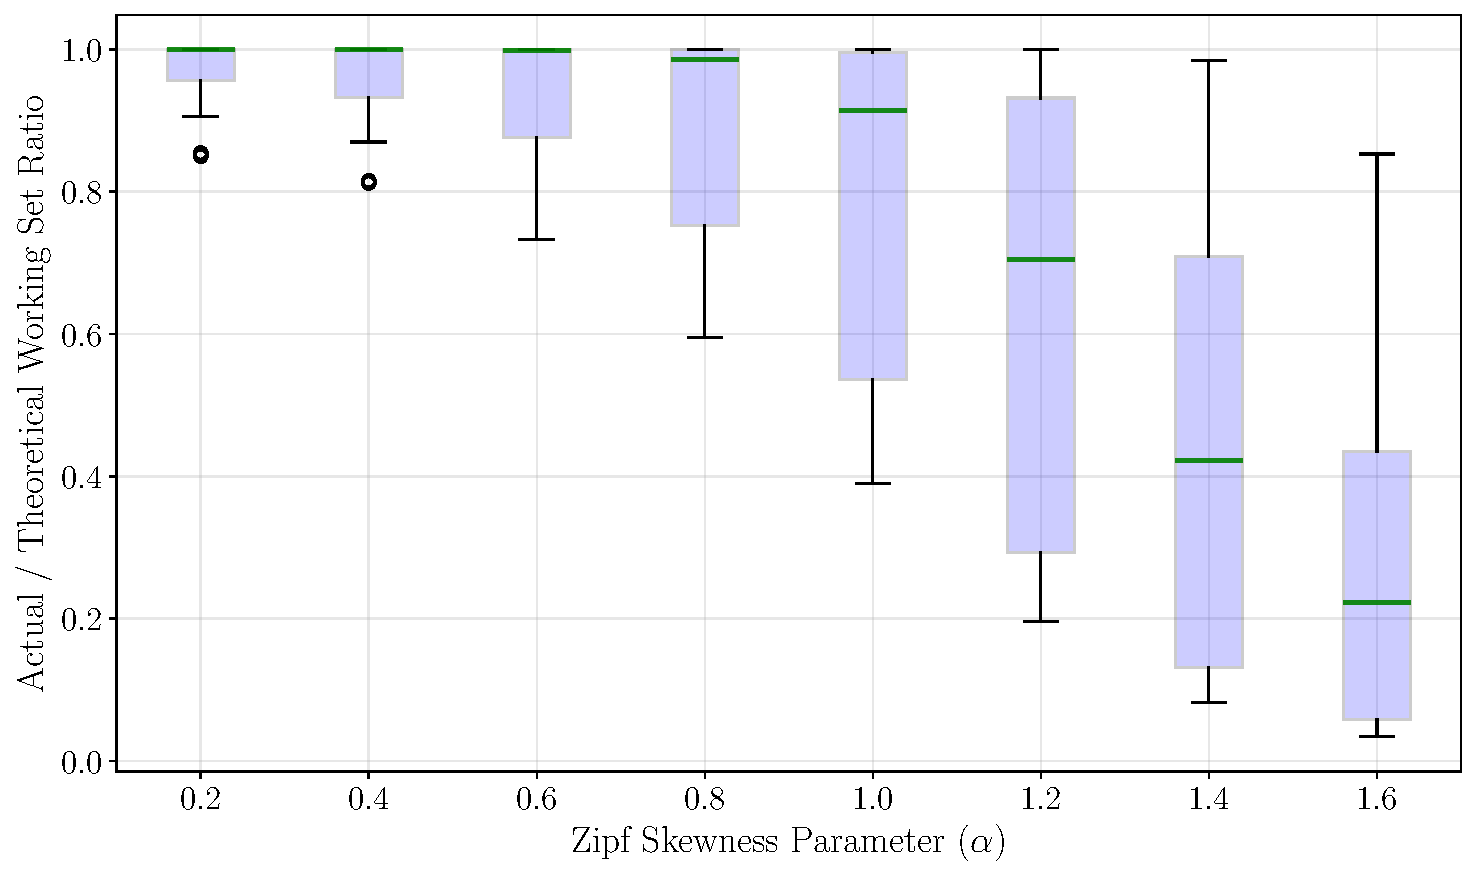
\includegraphics[width=0.8\linewidth]{figures/workloads/boxplot_alpha_vs_actual_theoretical_ratio.pdf}
    \label{fig:boxplot-actual-theoretical-ratio}
\end{figure}

From \Cref{fig:boxplot-actual-theoretical-ratio}, we observe that the skewness parameter $\alpha$ has a significant impact on the actual working set size generated. As $\alpha$ increases, the median ratio of the actual to the theoretical working set size decreases sharply. For a low skewness ($\alpha=0.2$), the median ratio is close to 1, indicating that most of the theoretical working set is captured. However, for a high skewness ($\alpha=1.6$), the median ratio drops below 25\%.

This phenomenon is due to the nature of sampling from a highly skewed distribution. A larger $\alpha$ means the distribution is more uneven, with a small number of items accounting for the majority of requests, while a long tail of very rare items exists. When a limited number of requests are sampled, it becomes increasingly difficult to encounter all of these rare items, leading to a smaller actual working set compared to the theoretical one.

Furthermore, we can see that a higher $\alpha$ value not only decreases the median ratio but also significantly increases the spread of the working set sizes, as evidenced by the widening interquartile range (IQR). For example, the less skewed distribution with $\alpha=0.2$ shows an IQR of around 1.5, while this IQR drastically increases to 8 for a more skewed distribution with $\alpha=1.6$. This wider spread suggests that for highly skewed distributions with large values for $\alpha$, the actual working set size can be highly variable depending on the specific sampling, highlighting the instability of the working set under these conditions.




%%%%%%%%%%%%%%%%%%%%%%%%%%%% CACHE SIMULATIONS

\section{Cache Simulations}\label{res:cache-sim}

This section outlines the experimental findings gathered from the cache simulations performed. We investigate findings regarding the generate miss ratio distribution of each algorithm before investigating the effects of the Zipfian skewness parameter $\alpha$ and the relative cache size on the measured miss ratios.

\subsection{Miss Ratio Distribution}\label{results:miss-ratio-distribution}

\outline{miss ratio distribution by algorithm}

As discussed in \Cref{subsec: cache-simulations}, a total of 28,371 cache simulations using unique configurations were performed on each algorithm. The miss ratio distribution for each algorithm (FIFO, LRU, SIEVE) is presented in the boxplot in \Cref{fig:miss-ratio-distribution}, with relevant miss ratio statistics outlined in \Cref{tab: miss_ratio_stats}.

\begin{table}[h!]
    \centering
    \caption{Summary of Cache Algorithm Miss Ratio Statistics}
    \label{tab: miss_ratio_stats}
    \begin{tabular}{l r r r r r r r r}
        \toprule
        \textbf{Algorithm} & \textbf{Mean} & \textbf{Median} & \textbf{Std Dev} & \textbf{Min} & \textbf{Max} & \textbf{Q1} & \textbf{Q3} & \textbf{IQR} \\
        \midrule
        FIFO & 0.6523 & 0.7688 & 0.3355 & 0.0111 & 1.0000 & 0.3420 & 0.9733 & 0.6313 \\
        LRU & 0.6324 & 0.7399 & 0.3469 & 0.0089 & 1.0000 & 0.2929 & 0.9724 & 0.6795 \\
        SIEVE & 0.5909 & 0.6483 & 0.3491 & 0.0088 & 1.0000 & 0.2464 & 0.9472 & 0.7008 \\
        \bottomrule
    \end{tabular}
\end{table}

\begin{figure}[h!]
    \centering
    \caption{Miss Ratio Distribution by Algorithm. The {\color{red}\textbf{red}} line represents the median.}
    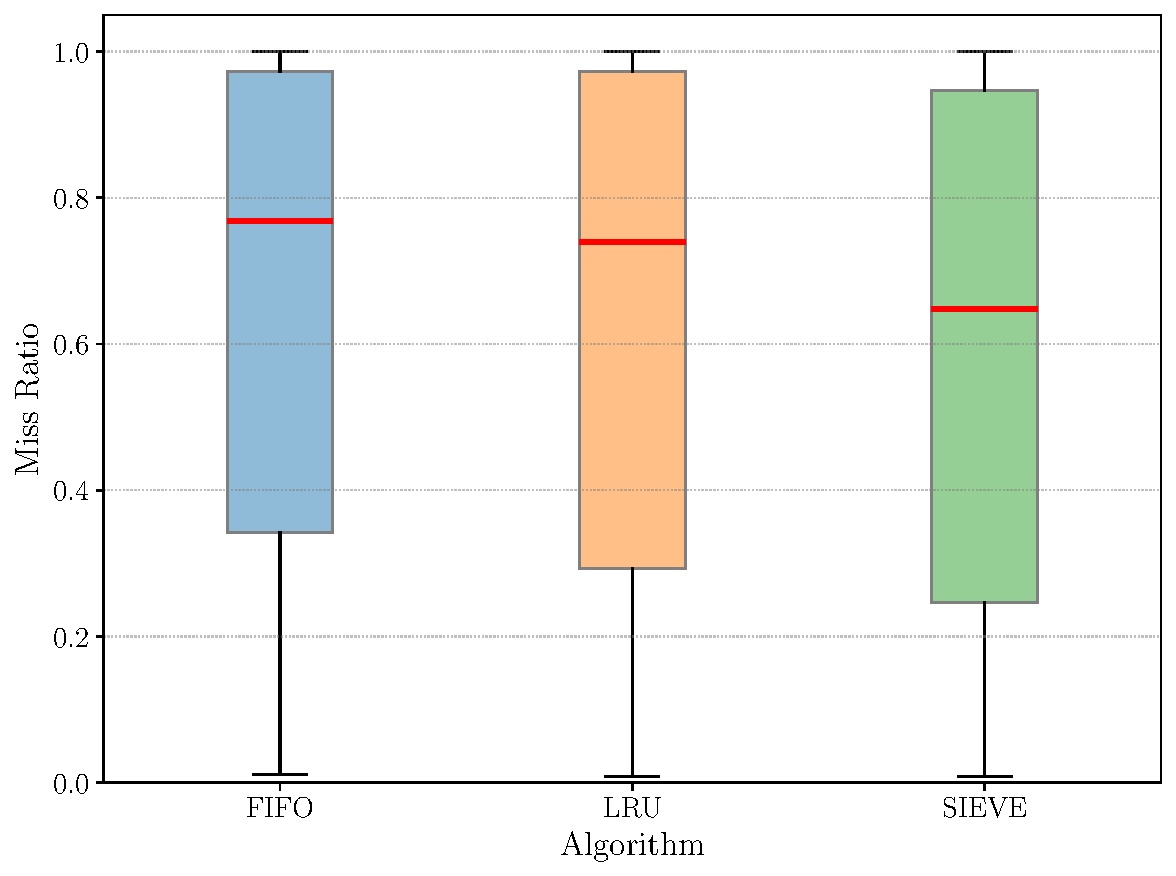
\includegraphics[width=0.6\linewidth]{figures/simulations/miss_ratio_distribution_no_title.pdf}
    \label{fig:miss-ratio-distribution}
\end{figure}

Based on the miss ratio boxplot (\Cref{fig:miss-ratio-distribution}) and accompanying table (\Cref{tab: miss_ratio_stats}) with relevant statistics, there is a clear performance hierarchy among the algorithms, with SIEVE generally outperforming the others. The median miss ratios show this trend: with a median miss ratio of 0.6483, SIEVE demonstrates a measurable advantage to its competitors, with LRU's median miss ratio being approximately 14.13\% higher and FIFO about 18.59\% higher than SIEVE's. This confirms that SIEVE, on average, handles all Zipf-like workloads, regardless of parameters, more efficiently than LRU and FIFO.

The mean miss ratios support this finding. SIEVE has a mean of 0.5909, which is lower than LRU (0.6324) and FIFO (0.6523). This suggests that SIEVE's performance is consistently better across the full range of simulations, followed by LRU.

All three algorithms exhibit a wide range of performance. The standard deviations are all relatively high (around 0.34), and the interquartile ranges (IQR) are broad, suggesting that the miss ratio for any given algorithm can vary significantly depending on the specific workload configuration. For example, all three algorithms have a minimum miss ratio close to zero and a maximum of 1.0, highlighting their sensitivity to factors like Zipfian skewness and relative cache size. Nevertheless, it is interesting to observe that SIEVE demonstrates the highest variability compared to the baselines, with slight differences in its standard deviation: 3.89\% greater than FIFO and 0.64\% greater than LRU.

Though all algorithms show a similar high degree of variability, SIEVE demonstrates a measurable advantage in terms of both median and mean miss ratio performance, indicating its strength when applied to Zipf-like distributions. Nevertheless, it is interesting to further investigate the cause for this high variability of miss ratios among all algorithms.

\subsection{Effect of Zipfian Skewness Parameter ($\alpha$) on Miss Ratio}\label{results:alpha-miss-ratio}

\outline{miss ratio vs. alpha}

The large variability in miss ratios can be directly linked to changes in the Zipfian skewness parameter ($\alpha$) used during workload generation. \Cref{fig:miss-ratio-vs-alpha} demonstrates the effect of $\alpha$ on the miss ratio. The exact values obtained for the mean miss ratio can be found in \Cref{appendix:mean-miss-ratio}.

\begin{figure}[h!]
    \centering
    \caption{Miss Ratio vs. Zipf Skewness Parameter $\alpha$}
    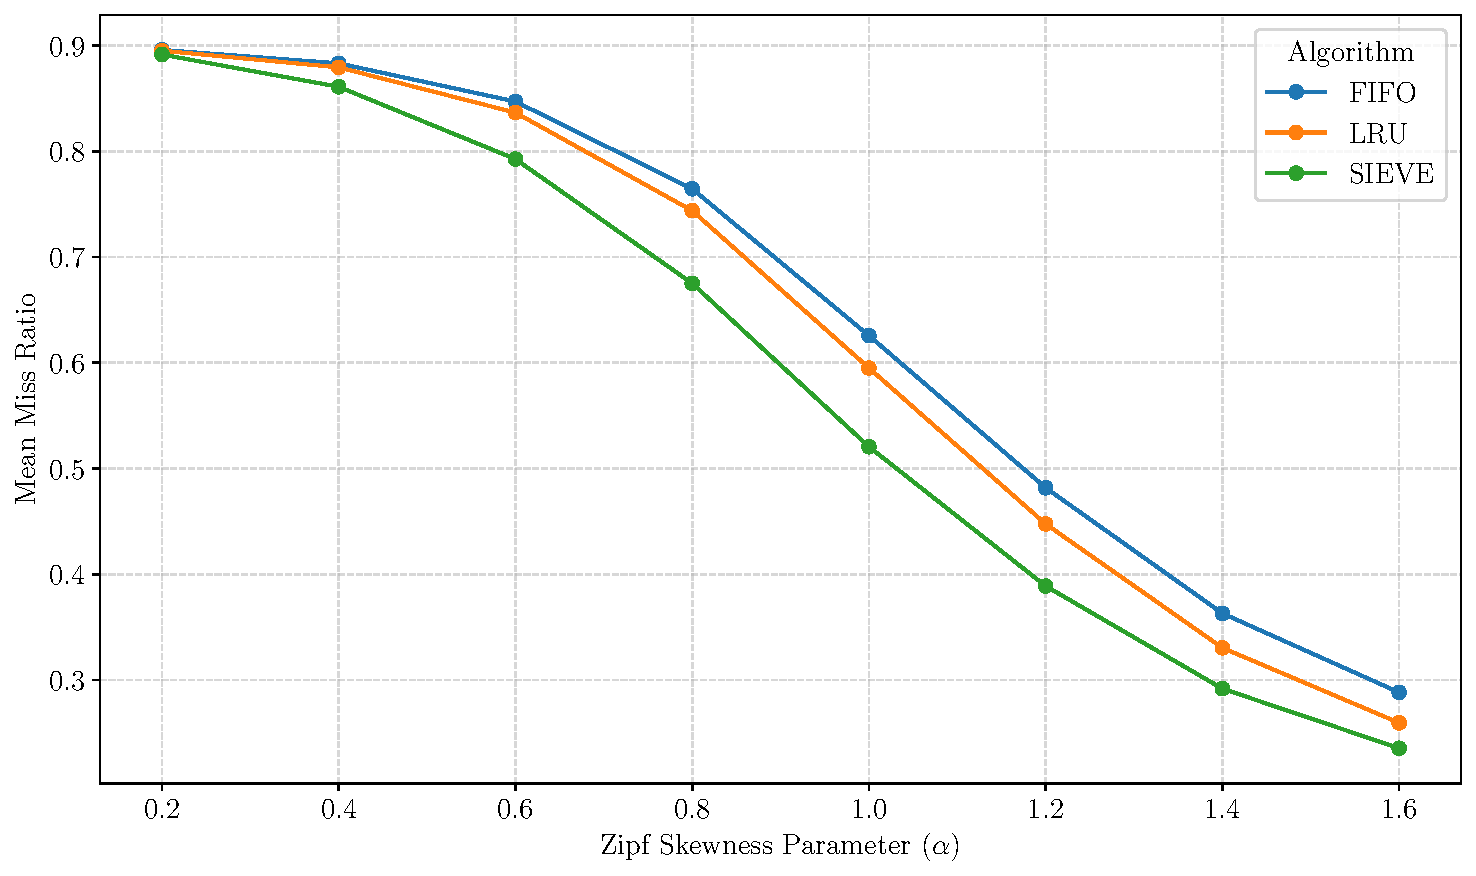
\includegraphics[width=0.8\linewidth]{figures/simulations/miss_ratio_vs_alpha_no_title.pdf}
    \label{fig:miss-ratio-vs-alpha}
\end{figure}

From \Cref{fig:miss-ratio-vs-alpha}, we can observe that, regardless of the algorithm used, the graph follows a downward-sloping curve. This demonstrates a crucial relationship: as $\alpha$ increases, the miss ratio decreases. This is a direct consequence of the nature of a Zipfian distribution: higher $\alpha$ values result in a more skewed distribution, where a small number of items are requested far more frequently. This concentration of requests on a few popular items leads to a greater number of cache hits and, consequently, a lower overall miss ratio.

When considering the performance of the different algorithms in \Cref{fig:miss-ratio-vs-alpha}, SIEVE consistently outperforms LRU and FIFO across all tested $\alpha$ values. This finding aligns with the general miss ratio distribution results discussed in \Cref{results:miss-ratio-distribution}, where SIEVE exhibited the lowest median miss ratio. The performance gap between SIEVE and the other algorithms is most pronounced in the mid-range of $\alpha$ values, particularly from $\alpha=0.8$ to $\alpha=1.2$. SIEVE's performance advantage is more visually apparent in \Cref{fig:sieve-advantage}, which plots the percentage advantage in miss ratio that SIEVE holds over FIFO and LRU.

\begin{figure}[h!]
    \centering
    \caption{Miss Ratio Performance Advantage of SIEVE Algorithm}
    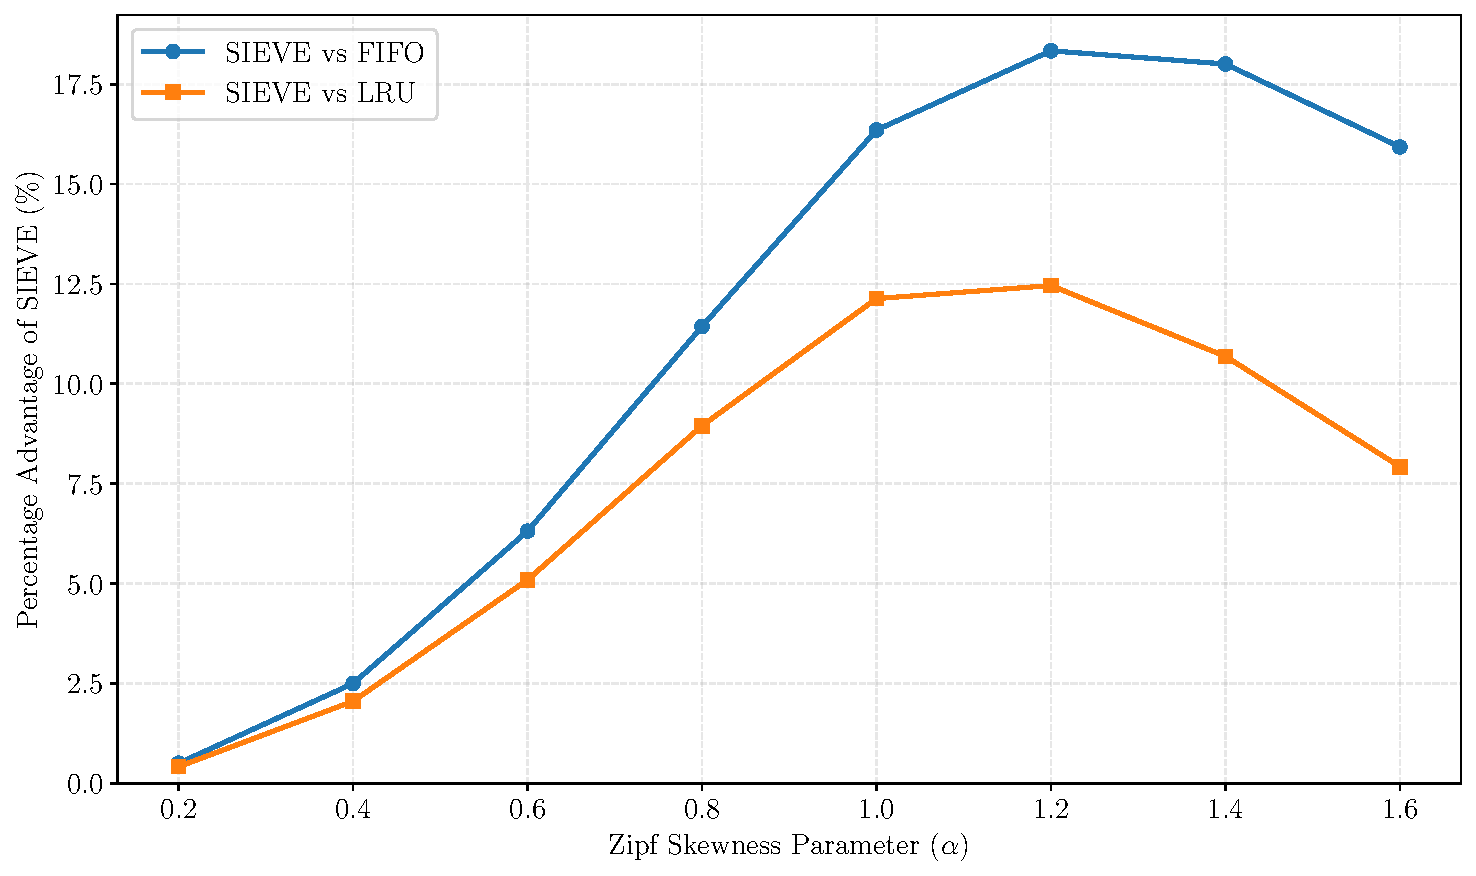
\includegraphics[width=0.8\linewidth]{figures/simulations/sieve_advantage_no_title.pdf}
    \label{fig:sieve-advantage}
\end{figure}

\Cref{fig:sieve-advantage} clearly shows that SIEVE's outperformance is not uniform. The miss ratio advantage peaks in the mid-range of $\alpha$ values. Specifically, the maximum advantage over LRU is approximately 13.12\% at $\alpha=1.2$, while the maximum advantage over FIFO is approximately 19.29\% at the same $\alpha$ value. This suggests that SIEVE is particularly effective at managing highly skewed workloads, where a balance is needed between caching the few very popular items and the large number of less popular items. As the skewness becomes extremely high (at $\alpha=1.6$) or low (at $\alpha=0.2$), the performance differences between the algorithms become less significant.

\subsection{Effect of Relative Cache Size on Miss Ratio}\label{results:miss-ratio-vs-relative-cache-size}

\outline{miss ratio vs. relative cache size}

Aside from the Zipfian skewness parameter $\alpha$ having a notable effect on the miss ratio of all algorithms, the relative cache size also has a significant impact. \Cref{fig:miss-ratio-cache-size} demonstrates a meaningful relationship between the relative cache sizes and the resulting mean miss ratio measured. The specific values measured can be found in \Cref{tab:miss_ratio_data}.

\begin{figure}[h!]
    \centering
    \caption{Miss Ratio vs. Relative Cache Size}
    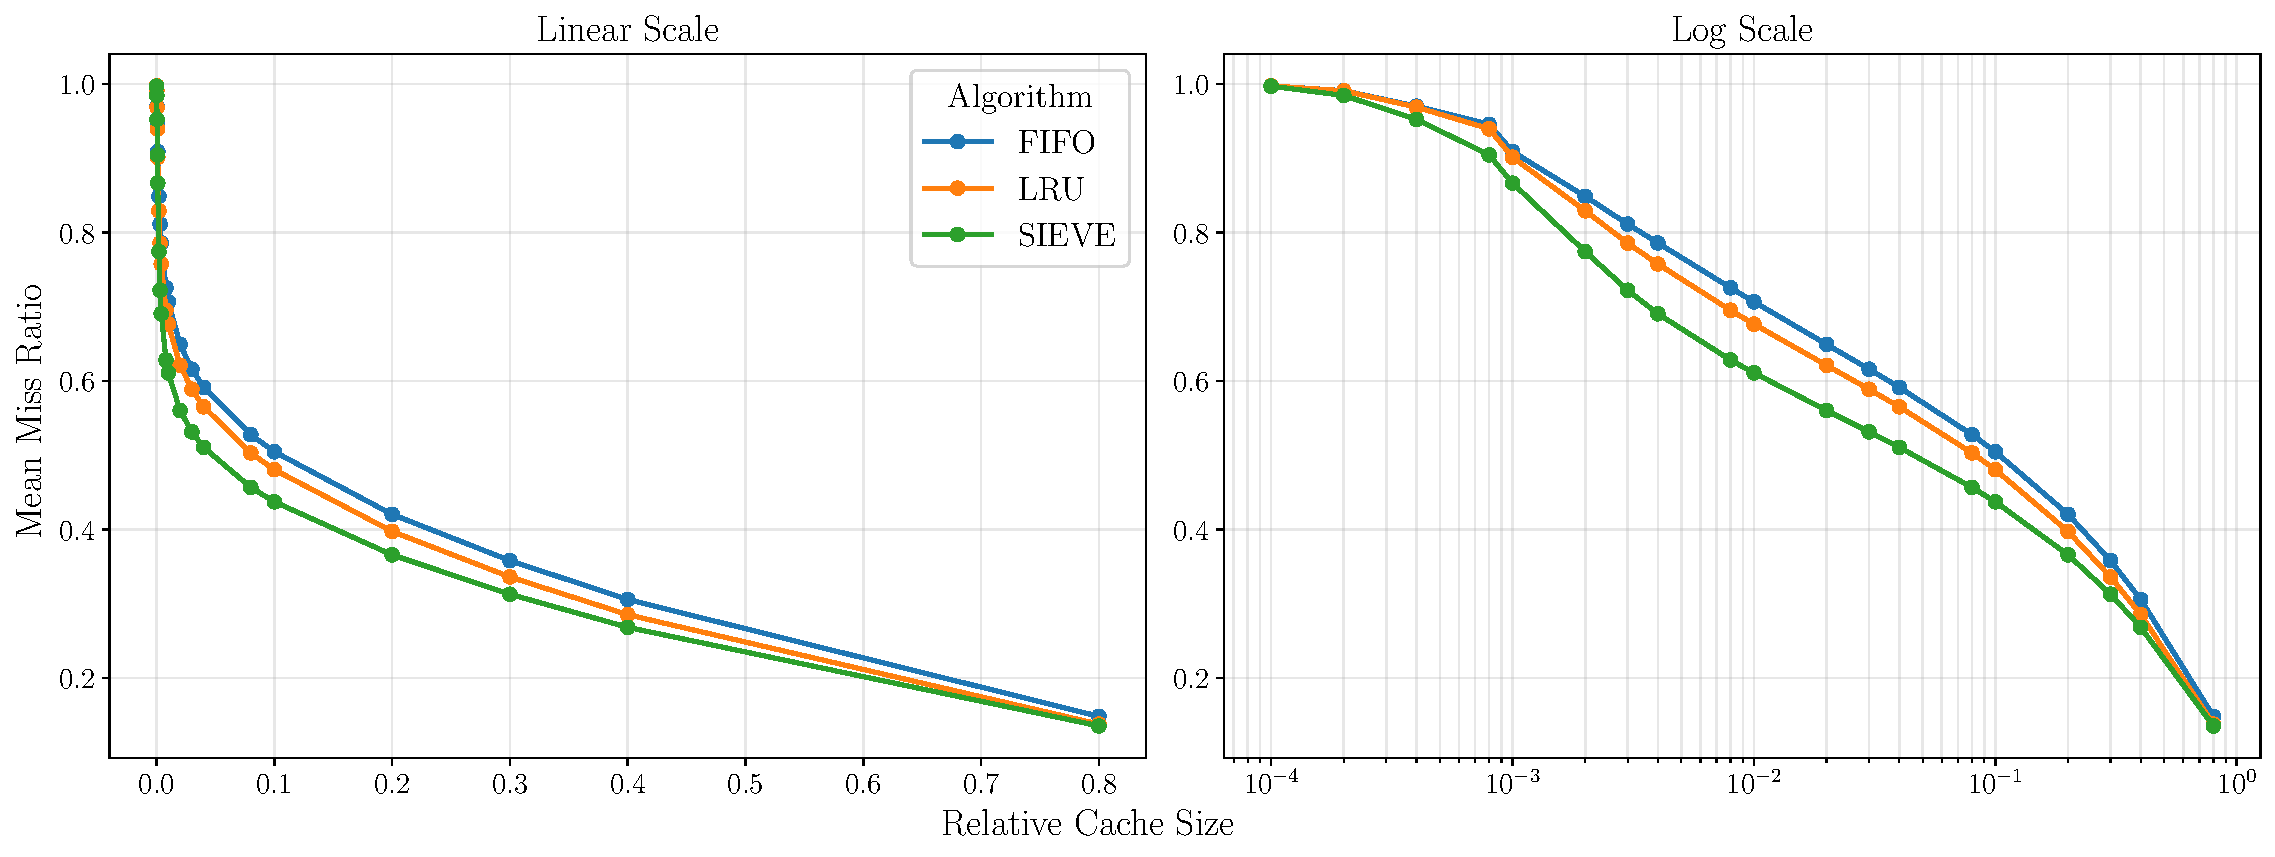
\includegraphics[width=\linewidth]{figures/simulations/miss_ratio_vs_cache_size_both.pdf}
    \label{fig:miss-ratio-cache-size}
\end{figure}

As shown in the linear scale plot in \Cref{fig:miss-ratio-cache-size}, the mean miss ratio consistently decreases with increasing relative cache size. However, the rate of this decrease is highly non-linear. The initial sharp drop in the miss ratio for relative cache sizes from 0 to approximately 0.04 indicates that small increases in cache size yield significant performance improvements, from a mean miss ratio of 0.9971 to 0.5107 for SIEVE.

Beyond a relative cache size of 0.1, the rate of improvement diminishes considerably. For example, increasing the relative cache size from 0.1 to 0.8 results in a much smaller reduction in miss ratio, dropping from 0.4374 to 0.1354 for SIEVE. This suggests a clear point of "diminishing returns" where further increases in cache size offer only marginal performance gains. The log scale plot on the right further highlights this non-linear relationship more clearly, visually stretching out the initial region of rapid performance gain and compressing the later region where gains are minimal.

Furthermore, when considering the relative performance of the three cache primitives, we see that SIEVE consistently maintains the lowest mean miss ratio across all relative cache sizes. For example, at a relative cache size of 0.2, SIEVE's miss ratio is 7.95\% better than LRU's and 12.98\% better than FIFO's.

\subsection{Combined Effect of $\alpha$ and Relative Cache Size on Miss Ratio}

\outline{miss ratio heat map}

The results demonstrated above, in \Cref{results:alpha-miss-ratio} and \Cref{results:miss-ratio-vs-relative-cache-size} both reveal that independent of $\alpha$ and the relative cache size, SIEVE consistently outperforms LRU and FIFO. The heatmap from \Cref{fig:miss-ratio-heatmap} reinforces these findings by displaying the meaningful relationship between $\alpha$, the relative cache size, and the resulting mean miss ratio measured. Each data point on the plot represents the mean miss ratio for a specific combination of $\alpha$, relative cache size, and caching algorithm (FIFO, LRU, and SIEVE).

\begin{figure}[h!]
    \centering
    \caption{Mean Miss Ratio vs. Zipf Skewness Parameter ($\alpha$) and Relative Cache Size}
    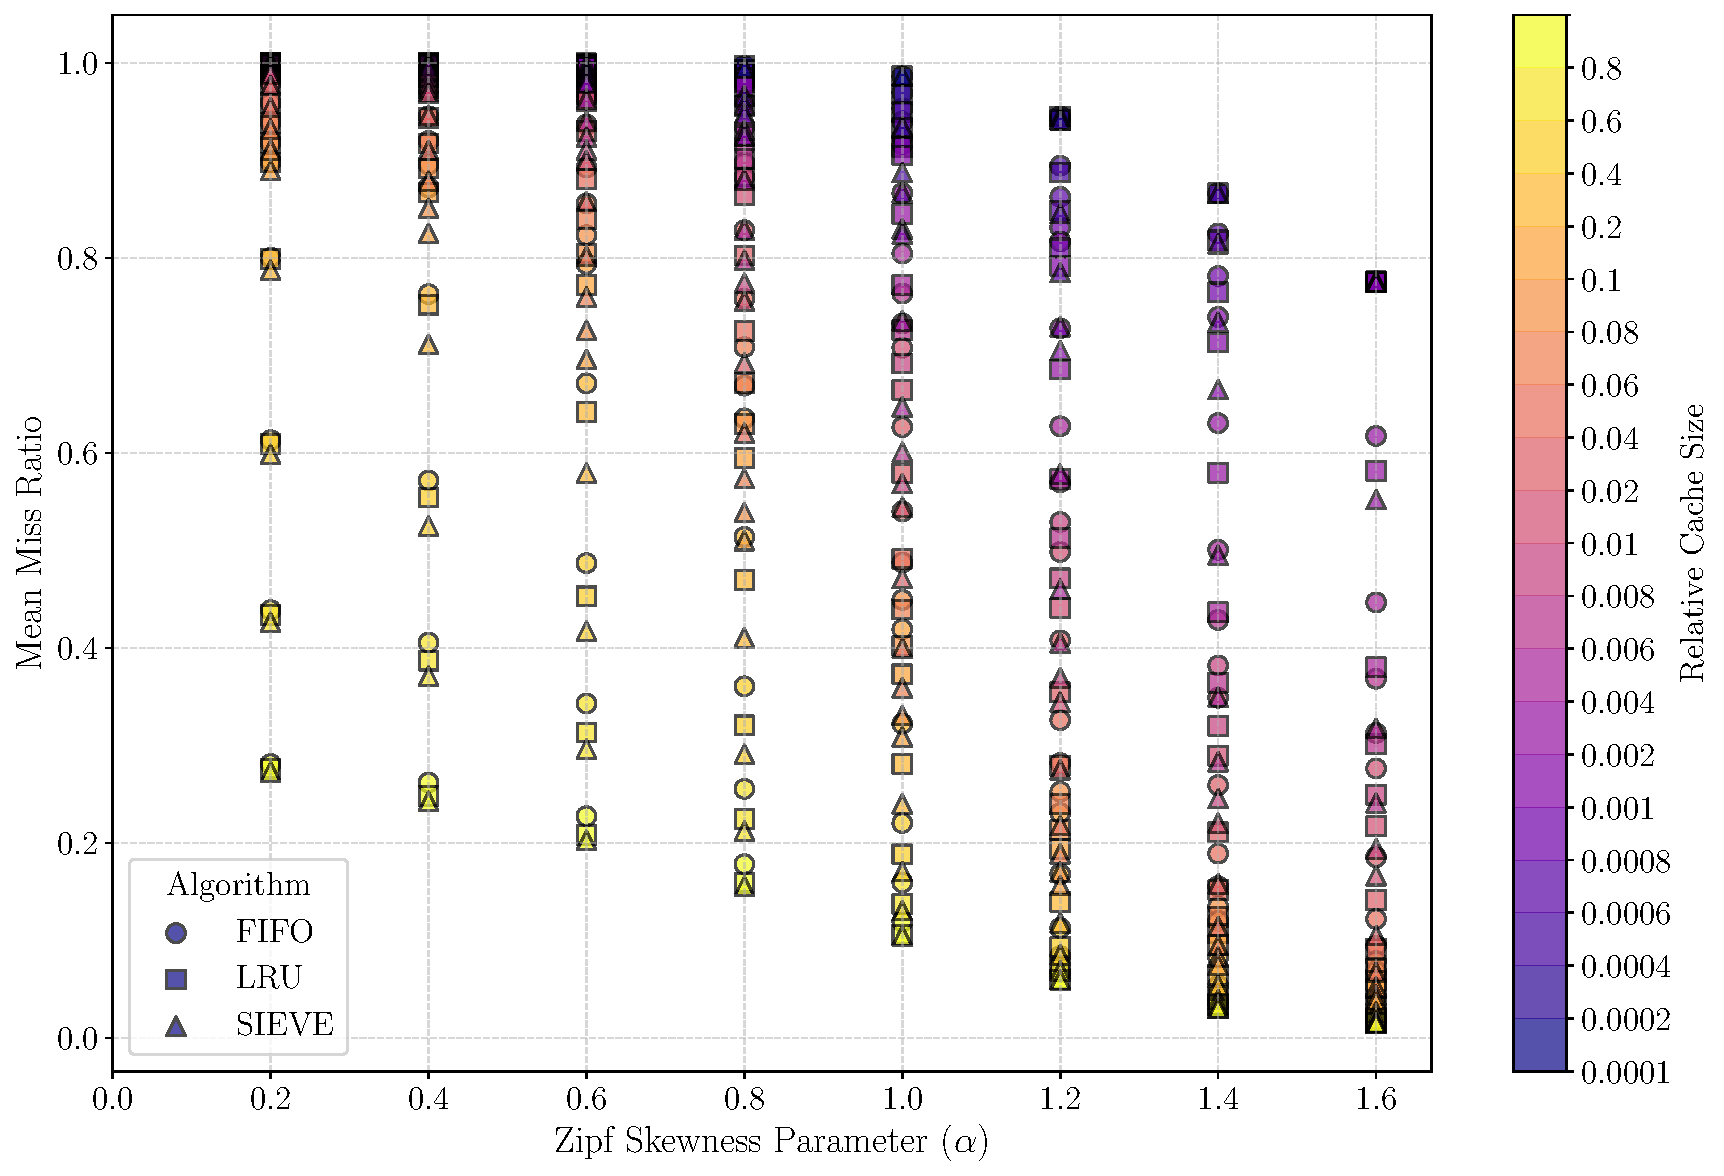
\includegraphics[width=\linewidth]{figures/simulations/miss_ratio_heat_map_no_title.pdf}
    \label{fig:miss-ratio-heatmap}
\end{figure}

A clear visual pattern emerges from the data demonstrated in \Cref{fig:miss-ratio-heatmap}: an inverse relationship between the miss ratio to $\alpha$ and the relative cache size. The larger cache sizes (yellow and light orange points) consistently result in a lower miss ratio across all $\alpha$ values. The most significant reduction in miss ratio occurs as the cache size increases, particularly in the mid-range of $\alpha$ values, where the workload is skewed enough to be captured by a reasonably sized cache, but not so extreme that a tiny cache is sufficient. The consistent vertical spread of points at each $\alpha$ value reinforces the strong influence of cache size on performance. This finding highlights the large impact that cache size has on the efficiency of any cache eviction algorithm. However, further research is required to determine the optimal trade-off between efficiency (as measured by miss ratio) and throughput, as both are critical metrics for overall system performance.
\newpage\chapter{Evaluation}
\newpage\chapter{Conclusion}

\section{Future Work}

\outline{Ideas for future work}

- test with proprietary traces

- more traces need to be available for use! (cite twitter-analysis here)

- running same algorithms on different production traces grouped by use case, and seeing whether there are trends there. for example, social media trends could be very different to others maybe

- looking at throughput as well, since not only efficiency matters lol
% \urlstyle{tt}
% \begin{otherlanguage}{australian}
% \setlength\bibitemsep{.2em}
% \printbibliography
% \end{otherlanguage}

\renewcommand{\bibname}{References}
\bibliographystyle{plain}
\bibliography{resources/references.bib}

\end{document}
